\chapter{Methodology}

\begin{figure}[htp]
    \centering
    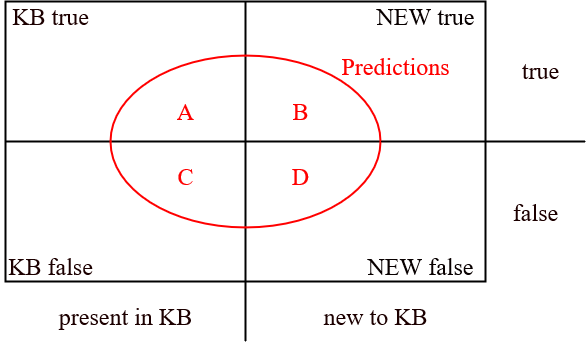
\includegraphics[width=10cm]{figures/kb_venn.png}
    \caption{KB prediction under incompleteness}
\end{figure}

\begin{figure}[htp]
    \centering
    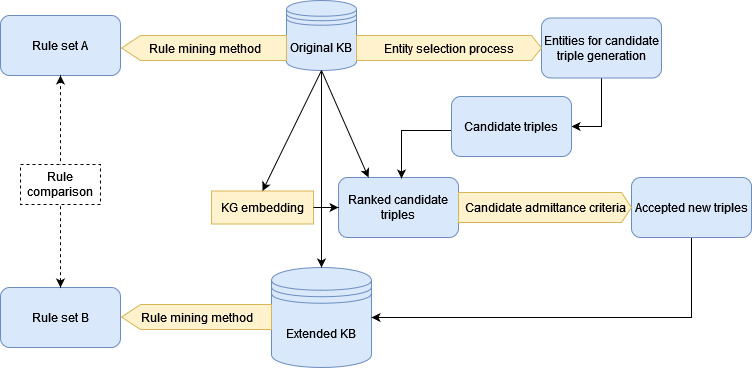
\includegraphics[width=12cm]{figures/ontology_mining_pipeline.jpg}
    \caption{KB prediction under incompleteness}
\end{figure}


TODO: write about your config file.

\section{Knowledge Graph Datasets}
While there are many large KGs publicly available, they are often quite complex in the number of different relations and entities used. Since we are mining rules over relations, the relational aspect of the KGs used was kept simple. By limiting the number of relations used in the KGs the resulting rules mined won't be overly diverse, and therefore easier for a human to understand evaluate. Two different datasets were used to conduct the experiments, both of which had been limited to contain only six different types of relations.


\subsection{Wikidata5M - family KG}
Wikidata5M is a KG dataset containing over 20 million triples with over 800 types of relations. It combines information from the Wikidata KG with Wikipedia pages \cite{wang2019kepler}. Wikidata5M uses the same identifier system as Wikidata, where each entity and relation is assigned a unique ID. The IDs of entities are prefixed with \texttt{Q} and those of relations with \texttt{P}. For example the following line \\
\centerline{\texttt{\href{https://www.wikidata.org/wiki/Q146}{Q146} \quad \href{https://www.wikidata.org/wiki/Property:P279}{P279} \quad  \href{https://www.wikidata.org/wiki/Q39201}{Q39201}}} \
corresponds to \textless\texttt{\href{https://www.wikidata.org/wiki/Q146}{house cat}, \href{https://www.wikidata.org/wiki/Property:P279}{subclass of}, \href{https://www.wikidata.org/wiki/Q39201}{pet}}\textgreater, where each entity has a corresponding Wikipedia page.
This dataset was chosen due to its size and because it contained family-related information. Rules about family structure are well-known and easy to comprehend. For example the simple rule $parent(a, b) \Rightarrow  child(b, a)$ would be implicitly represented in the data of such a subset.
\begin{lstlisting}[language=Python, caption={Python dictionary converting family predicate IDs to their names},captionpos=t, label={family_predicated_dict}]
family_predicates_dict = {
    'P40': 'child', 
    'P22' : 'father', 
    'P25' : 'mother',
    'P26' : 'spouse', 
    'P1038' : 'relative', 
    'P3373' : 'sibling', 
}
\end{lstlisting}

After filtering out all triples that did not use one of the six selected family predicates, the IDs were converted to meaningful names so that the resulting rules mined would be easily readable. The python dictionary listen in \ref{family_predicated_dict} shows the chosen predicates. A few other family predicates were considered, but did not have as many corresponding data points or were too similar to other selected predicates. Predicates such as \texttt{grandchild} or \texttt{sister} are also not currently used in Wikidata, and from a discussion in the Wikidata community it seems that all properties considered redundant were removed \cite{kinship_discussion}. For the experiments Pykeen's distribution of the dataset was used \cite{ali2021pykeen}. The resulting subset of Wikidata5M contained around 250 000 triples and will henceforth be refferred to as the \textit{family KG}. 

\subsection{WN18RR}
WN18RR is a smaller KG dataset with 93 003 triples and only 11 relations \cite{dettmers2018convolutional}. It is based on the WN18 dataset, which contains triples scraped from WordNet, a lexical database for English \cite{wordNet}. It was found that there was information leakage between the training and test set of WN18 through inverse relations, where a large number of test triples could be identified simply by inverting triples in the training set \cite{toutanova2015observed}. WN18RR addresses this issue. In WordNet nouns, verbs, adjectives and adverbs are grouped into sets of semantic synonyms called \textit{synsets}. An example if a synset is \textit{\textbf{cat, true cat} (feline mammal usually having thick soft fur and no ability to roar)}. Synsets are connected to other synsets by semantic relations. The most commonly used relation in WN18RR is \texttt{hypernym}. A synset \texttt{X} is a hypernym of synset \texttt{Y}, if every \texttt{Y} is a kind of \texttt{X}. For example the triple 
\centerline{\texttt{02121808 \quad hypernym \quad 02121620}}
represents the information that the synset \texttt{cat} is a hypernym of the synset \texttt{house cat}. Or more simply phrased: \textit{All house cats are cats}.

\begin{table}[ht]
\centering
\begin{tabular}{|c|c|c|}
\hline
& \textbf{Relation} & \textbf{Frequency}\\
\hline
\multirow{6}{*}{\rotatebox[origin=c]{90}{Included}} &hypernym & 36873\\
&derivationally related form & 31865\\
&member meronym & 7912\\
&has part & 5131\\
&synset domain topic of & 3328\\
&instance hypernym & 3118\\
\hline
\multirow{5}{*}{\rotatebox[origin=c]{90}{Excluded}}&also see & 1396\\
&verb group & 1220\\
&member of domain region & 981\\
&member of domain usage & 673\\
&similar to & 86\\
\hline
\end{tabular}
\caption{Frequency of relations in WN18RR KG and whether they were included in the final KG}
\end{table}

WN18RR was chosen because the number of relations needed to be limited, and with a dataset already containing few relations most of it could be included. By taking all triples containing one of the six most frequent relations, in total 88227 datapoints, 95\% of WN18RR was used. This was intended to produce a more complete KG. For the experiments AmpliGraph's distribution of the dataset was used \cite{ampligraph}.

\section{KG embeddings}
The library AmpliGraph was used for the KG embedding models. AmpliGraph is an open source library based on Tensorflow. The library provides many different KG embedding models, metric calculators and also allows for the prediction of new triples in KGs. Three different KG embedding methods were selected: TransE, DistMult and ComplEx. AmpliGraph also provides a baseline model, which the three selected models were compared to. 

Each embedding model has a number of hyperparameters that could be optimised. As the search space grows it has been shown that random search is more optimal than grid search, where each combination needs to be tested \cite{bergstra2012random}. Due to limited computational resources, this approach to hyperparameter optimisation was selected. It is not an optimal approach, but serves as a practical and effective solution that measures well against more sophisticated methods such as Baysian optimisation \cite{li2017hyperband}.

\begin{table}[]
\centering
\begin{tabular}{|l|l|}
\hline
\textbf{Hyperparameter}      & \textbf{Values}             \\ \hline
Batches count       & 50, 100                              \\ \hline
Epocs               & 50, 100                          \\ \hline
k                   & 50, 100, 200                     \\ \hline
eta                 & 5, 10, 15                            \\ \hline
Pairwise loss margin    & 0.5, 1, 2                    \\ \hline
%Regularizer         & LP                             \\ \hline
%Learning rate       & Random number in range(0.0001, 0.01) \\ \hline
\end{tabular}
%\label{{hyperparameter_table}
\caption{Hyperparameter values to search through in model selection.}
\end{table}

The AmpliGraph documentation was a main inspriation when deciding which hyperparameters to focus on. It was for example stated in the documentation that they recieved the best results with the adam optimizer, therefore other optimisers were not considered in the hyperparameter search \cite{ampligraph_documentation}. Since pairwise hinge loss has been shown to be an adequate loss function for both TransE, DistMult and ComplEx, it was chosen and other functions were not explored in the hyperparameter search \cite{mohamed2019loss}. Different values for the  pairwise loss margin were however included in the search. For each hyperparameter combination a learning rate randomly chosen in the range of 0.0001 - 0.01 was selected. 

For the implementation of model selection AmpliGraph's \texttt{select\_best\_mode\_ranking} was used. It is a model selection routine that allows for both grid and random search. At the end of each model selection process, the final model for each embedding type is retrained on the concatenation of the train and validation set, before it is eventually evaluated on the test set. As the training data only contains positive examples, negative ones are generated. The \texttt{eta} hyperparameter denotes the number of negative examples generates at training for each positive example. In the training process corrupted triples are generated according to the strategy proposed on the paper in which TransE was introduced \cite{TransE}. This approach takes valid triples and replaces either the head or tail (but not both) with a random entity. TODO: remove, this has been written about(?)

\subsection{Model selection results}
% Please add the following required packages to your document preamble:
% \usepackage{multirow}
% \usepackage[normalem]{ulem}
% \useunder{\uline}{\ul}{}
\begin{table}[]
\centering
\begin{tabular}{|l||ccccc||ccccc|}
\hline
{\textbf{DATASET}}                 & \multicolumn{5}{c||}{\textbf{WN18RR}}                                                                                                                                               & \multicolumn{5}{c|}{\textbf{Family KG}}                                                                                                                            \\ \hline
\multirow{2}{*}{{\textbf{METRIC}}} & \multicolumn{1}{c|}{\multirow{2}{*}{\textbf{MR}}} & \multicolumn{1}{c|}{\multirow{2}{*}{\textbf{MRR}}} & \multicolumn{3}{c||}{\textbf{Hits@}}                                       & \multicolumn{1}{c|}{\multirow{2}{*}{\textbf{MR}}} & \multicolumn{1}{c|}{\multirow{2}{*}{\textbf{MRR}}} & \multicolumn{3}{c|}{\textbf{Hits@}}                                       \\ \cline{4-6} \cline{9-11} 
                                       & \multicolumn{1}{c|}{}                             & \multicolumn{1}{c|}{}                              & \multicolumn{1}{l|}{\textbf{1}} & \multicolumn{1}{l|}{\textbf{3}} & \multicolumn{1}{l||}{\textbf{10}} & \multicolumn{1}{c|}{}                             & \multicolumn{1}{c|}{}                              & \multicolumn{1}{l|}{\textbf{1}} & \multicolumn{1}{l|}{\textbf{3}} & \multicolumn{1}{l|}{\textbf{10}} \\ \hline
\textbf{Baseline}                      & 1                                                 & 1                                                  & 1                      & 1                      & 1                       & 1                                                 & 1                                                  & 1                      & 1                      & 1                       \\ 
\textbf{TransE}                        & 1                                                  & 1                                                  & 1                      & 1                      & 1                       & 1                                                 & 1                                                  & 1                      & 1                      & 1                       \\ 
\textbf{DistMult}                      & 1                                                 & 1                                                  & 1                      & 1                      & 1                       & 1                                                 & 1                                                  & 1                      & 1                      & 1                       \\ 
\textbf{ComplEx}                       & 1                                                 & 1                                                  & 1                      & 1                      & 1                       & 1                                                 & 1                                                  & 1                      & 1                      & 1                       \\ \hline
\end{tabular}
\caption{Results of selected models evaluated on test set.}
\end{table}

\begin{figure}[htp]
    \centering
    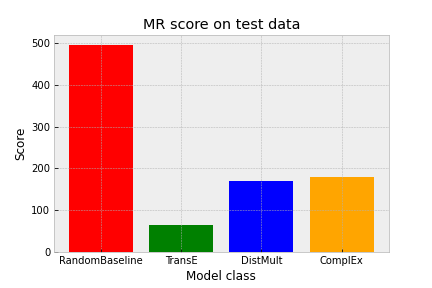
\includegraphics[width=12cm]{figures/model_selection/family_scores_1.png}
    \caption{KB prediction under incompleteness}
\end{figure}


\begin{figure}[htp]
    \centering
    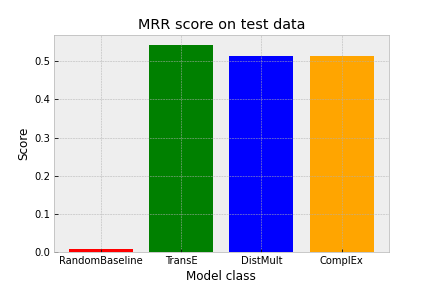
\includegraphics[width=12cm]{figures/model_selection/family_scores_0.png}
    \caption{KB prediction under incompleteness}
\end{figure}


\begin{figure}[htp]
    \centering
    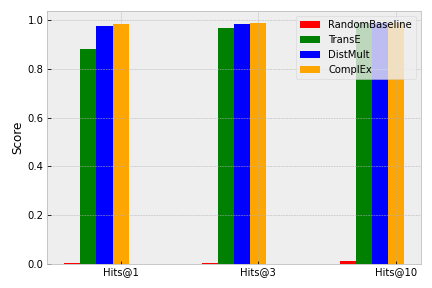
\includegraphics[width=12cm]{figures/model_selection/family_hit_scores.png}
    \caption{KB prediction under incompleteness}
\end{figure}


%epochs (int) – The iterations of the training loop.

%batches_count (int) – The number of batches in which the training set must be split during the training loop.

%k (int) – Embedding space dimensionality.

%loss : pairwise loss, with a margin of 0.5 set via the loss_params kwarg.

TODO: add results and write about them

\newpage

\section{KG extension}

The goal of KG extension is to add potentially true statements to the original KG. AmpliGraph does have an implementation for this, called \texttt{discover\_facts}, but for technical reasons it could not be used. The implementation used in this thesis does however follow the same strategy used in \texttt{discover\_facts}. It consists of two main parts:
\begin{enumerate}
    \item Candidate triple generation
    \item Ranking of generated candidates
\end{enumerate}
Once one has a set of ranked candidate triples all that remains is to decide what the minimum rank should be for a candidate to be added to the KG.


\subsection{Candidate triple generation}
Both WN18RR and the family KG contain too many entities for it to be possible to consider all possible triples when extending the KB. TODO: add exact numbers. There are only 6 types of relations in each dataset, but WN18RR and the family KG contain X and Y entities respectively. Therefore only a small subset of these entities can be included in the candidate generation. Four approaches were tested:
\begin{itemize}
    \item random selection
    \item the most frequent entities
    \item the least frequent entities
    \item probabilistic selection based on the frequency of the entities in the dataset
\end{itemize}
Once the entities were selected, all possible triples were generated with them and the six relations. The resulting candidate triples were then filtered such that no triples already included in the original KG also were candidates to the extension. Of course the more triples that are considered for the extension, the better the extension will be, but again computational limitations restricted this. After trying different candidate set sizes it was eventually decided that selecting 1000 entities for candidate triple generation was a feasible number. This meant that $ 1000 \times 6 \times 1000 = 6 \times 10^6 $ triples (minus those that already appeared in the KB) were considered for each KG extension.


\subsection{Candidate triple ranking}
As discussed in (TODO: add section) it is not easy to set a relative score to a triple, based on a KG embedding. Therefore candidate triples are ranked against corrupted triples. An accurate KG embedding model will rank well-suited candidates higher than the corrupted triples. Since only one side of each triple is corrupted at a time, the corrupted triples generated are compliant with the local closed world assumption. AmpliGraph's function \texttt{evaluate\_performance} evaluates the performance of a trained KG embedding model by ranking a set of test triples from the KG against a set of corrupted triples. One then evaluated the embedding model based on how good it is at ranking the positive test triples higher than the negative corrupted triples. By instead passing the set of candidate triples to \texttt{evaluate\_performance} these could be ranked instead. Once the candidates have been given ranks one simply needs to decide on a cutoff rank to consider the candidate as a true positive and add it to the KG.






\section{Rule mining and evaluation}
